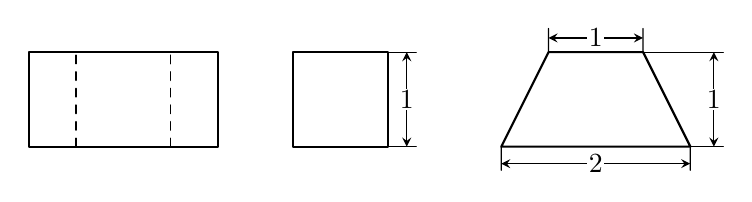
\begin{tikzpicture}[baseline,line cap=round,line join=round,>=stealth,scale=1.2]
  \tikzset{
    thickline/.style={line width=0.8pt},
    dimline/.style={line width=0.45pt},
  }

  % ==================== 正视图 ====================
  \draw[thickline] (0,0) rectangle (2,1);
  \draw[dashed,line width=0.6pt] (0.5,0) -- (0.5,1);
  \draw[dashed,line width=0.6pt] (1.5,0) -- (1.5,1);

  % ==================== 侧视图 ====================
  \def\sx{2.8}
  \draw[thickline] (\sx,0) rectangle (\sx+1,1);
  % Height 1 dimension on right
  \draw[dimline] (\sx+1,1) -- (\sx+1.3,1);
  \draw[dimline] (\sx+1,0) -- (\sx+1.3,0);
  \draw[<->,dimline] (\sx+1.2,0) -- (\sx+1.2,1) node[midway,fill=white,inner sep=0.5pt] {$1$};

  % ==================== 俯视图 ====================
  \def\tx{5.0}
  \coordinate (T_BL) at (\tx,0);
  \coordinate (T_BR) at (\tx+2,0);
  \coordinate (T_TR) at (\tx+1.5,1);
  \coordinate (T_TL) at (\tx+0.5,1);

  \draw[thickline] (T_BL) -- (T_BR) -- (T_TR) -- (T_TL) -- cycle;

  % Top base 1 dimension
  \draw[dimline] (T_TL) -- (\tx+0.5,1.25);
  \draw[dimline] (T_TR) -- (\tx+1.5,1.25);
  \draw[<->,dimline] (\tx+0.5,1.15) -- (\tx+1.5,1.15) node[midway,fill=white,inner sep=0.5pt] {$1$};

  % Bottom base 2 dimension
  \draw[dimline] (T_BL) -- (\tx,-0.25);
  \draw[dimline] (T_BR) -- (\tx+2,-0.25);
  \draw[<->,dimline] (\tx,-0.18) -- (\tx+2,-0.18) node[midway,fill=white,inner sep=0.5pt] {$2$};

  % Height 1 dimension on right
  \draw[dimline] (\tx+2,0) -- (\tx+2.35,0);
  \draw[dimline] (\tx+1.5,1) -- (\tx+2.35,1);
  \draw[<->,dimline] (\tx+2.25,0) -- (\tx+2.25,1) node[midway,fill=white,inner sep=0.5pt] {$1$};
\end{tikzpicture}
